\documentclass[a4paper,10pt]{article}

\usepackage{graphicx}
%opening
\title{Progress Report}
\author{Ewald Zietsman}
\date{January 2008}

\begin{document}

\maketitle

\section{Goal of the Project}

This project is an investigation of the rapid oscillations observed in the cataclysmic variable star EC2117-5417. High-speed photometric and high-speed spectroscopic observations were obtained using the SAAO 1.9m and Southern African Large Telescope (SALT) respectively during August 2006. The main goals of the project are to study the behaviour of Dwarf Nova Oscillations (DNOs) and long period DNOs (lpDNOs) during eclipse.


\section{Completed work}

\subsection{Observations}

Photometric and spectroscopic observations were obtained during August 2006. The photometric observations were made using the SAAO 1.9m telescope in Sutherland. Figure \ref{photometry} shows the lightcurves of EC2117-54 obtained during August 2006. During Run S7655 simultaneous spectroscopic observations were made using the Robert Stobie Spectrograph (RSS) on SALT. Figure \ref{SALT_Coverage} shows the extent of the SALT observations. The average spectrum observed using SALT is shown in figure \ref{average_spec}. 

\begin{figure}
 \centering
 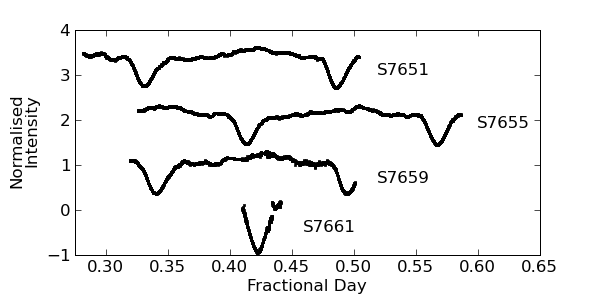
\includegraphics[width=0.8\columnwidth,bb=0 0 600 400]{../images/lightcurves.png}
 % lightcurves.png: 600x400 pixel, 72dpi, 21.17x14.11 cm, bb=0 0 600 400
 \caption{Photometric observations of EC2117-54 during August 2006. The lightcurves are vertically displaced by arbitrary amounts for display purposes}
 \label{photometry}
\end{figure}


\begin{figure}
 \centering
 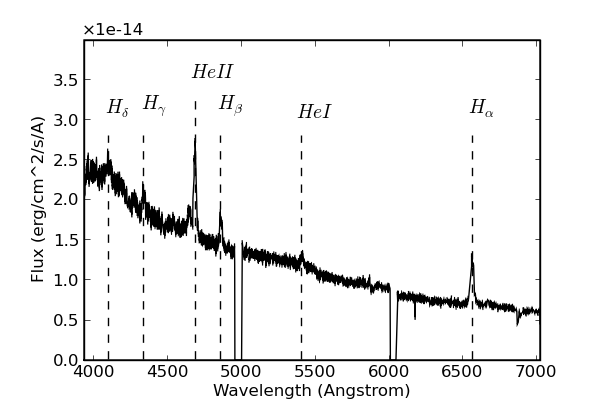
\includegraphics[bb=0 0 600 400,width=0.8\columnwidth]{../images/EC2117.png}
 % EC2117.png: 600x400 pixel, 72dpi, 21.17x14.11 cm, bb=0 0 600 400
 \caption{Average SALT spectrum of EC2117-54. The most prominent emission lines are marked.}
 \label{average_spec}
\end{figure}

\begin{figure}
 \centering
 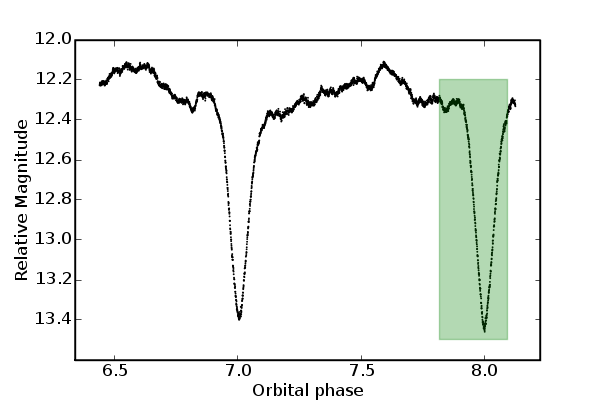
\includegraphics[bb=0 0 600 400,width=0.8\columnwidth]{../images/S7655_SALT_coverage.png}
 % EC2117.png: 600x400 pixel, 72dpi, 21.17x14.11 cm, bb=0 0 600 400
 \caption{Lightcurve of run S7655 and extent of SALT spectroscopy. The shaded area shows extent of SALT observations.}
 \label{SALT_Coverage}
\end{figure}


\subsection{Data Reductions}

All observational data have been reduced and are ready to be analysed. The photometric observations obtained during August 2006 have been reduced ``on-the-fly'' at the telescope using a custom data reduction pipeline written by Darragh O'Donoghue. The SALT spectroscopic data have been reduced using custom software utilising the \texttt{Python} language and the \texttt{IRAF} data reduction software.


\subsection{Data Analysis}
\subsubsection{Photometry}

Photometric data from 2003 were retrieved from the archive and have been included in the analysis. All photometric runs have been analysed in full for rapid oscillations the results have been catalogued. Software needed to be written to analyse the datasets since no standard software is available. 

The photometric runs were analysed using standard Fourier analysis techniques. Datasets were run through high-pass filters before being analysed for rapid oscillations in order to remove orbital variations. Digital Infinite Impulse Response (IIR) filters were used to accomplish this. Figure \ref{unflat} shows the periodogram of an unfiltered lightcurve. The periodogram is noisy and small amplitude oscillations cannot be identified. Figure \ref{flat} shows a filtered lightcurve and its periodogram. Small amplitude signals are now visible in the periodogram.

These techniques allow us to identify which lightcurves contain DNOs and lpDNOs. These oscillations are then identified in runs that contains eclipses i.e. when the cool bigger star moves in front of the small hot star. We then study the amplitude and phase changes of the oscillations throught the eclipses. Figure \ref{average_OC} shows the averaged amplitude and phase change during eclipse of all detected dwarf nova oscillations. A clear phase change can be seen during the eclipse (Time of minimum light is at orbital phase 1.0).


\begin{figure}
 \centering
 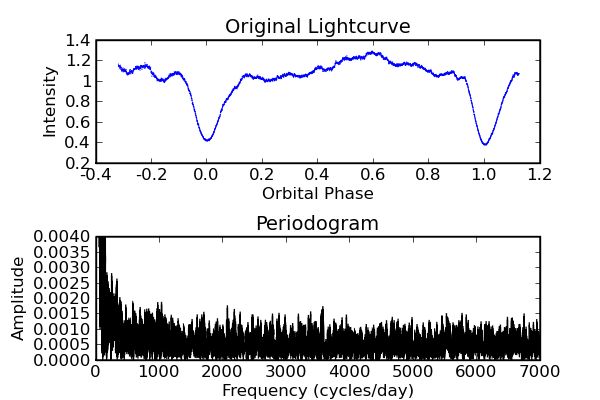
\includegraphics[bb=0 0 600 400,width=0.8\columnwidth]{../images/unflattened.png}
 % flattened.png: 600x400 pixel, 100dpi, 15.24x10.16 cm, bb=0 0 432 288
 \caption{Run S7651 before high-pass filtering and its periodogram. No short period oscillations can be discerned.}
 \label{unflat}
\end{figure}

\begin{figure}
 \centering
 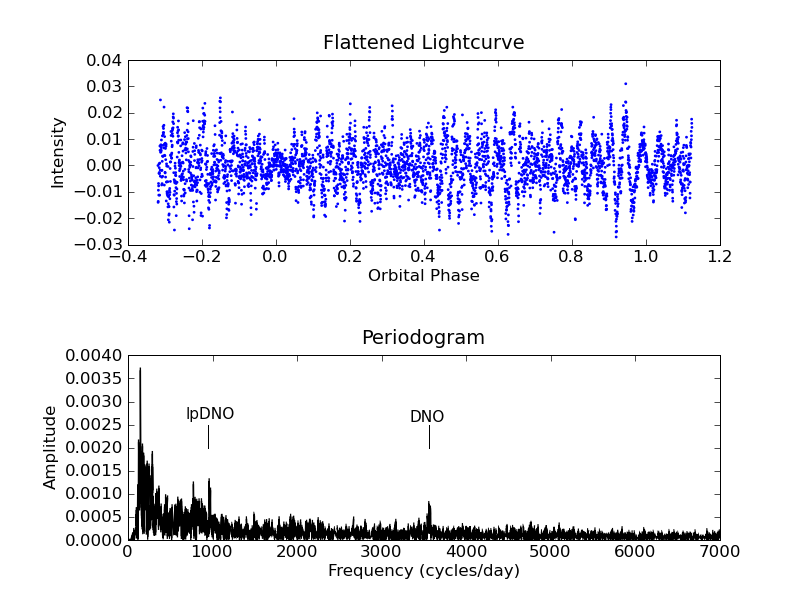
\includegraphics[bb=0 0 600 400,width=0.8\columnwidth]{../images/flattened.png}
 % flattened.png: 600x400 pixel, 100dpi, 15.24x10.16 cm, bb=0 0 432 288
 \caption{Run S7651 after high-pass filtering and its periodogram. DNO and lpDNO peaks are now easily identified.}
 \label{flat}
\end{figure}


\begin{figure}
 \centering
 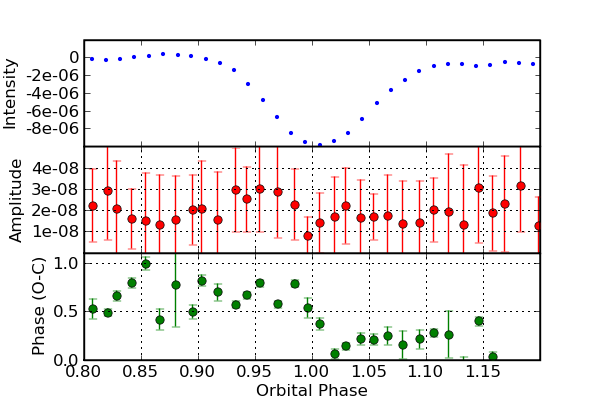
\includegraphics[width=0.8\columnwidth,bb=0 0 600 400]{../images/average_OC.png}
 % average_OC.png: 600x400 pixel, 100dpi, 15.24x10.16 cm, bb=0 0 432 288
 \caption{Average amplitude and phase of DNOs during eclipse.}
 \label{average_OC}
\end{figure}



\section{Incomplete work}

\subsection{Photometry}

A small number of refinements must be made to existing calculations.


\subsection{Spectroscopy}

The spectroscopic data needs to be analysed based on results obtained from photometric analysis. The spectroscopic data is fully reduced and calibrated and is ready for analysis.


\subsection{Analysis}

The observational findings must be discussed with supervisors. 


\subsection{Write-up}

The write-up is mostly complete except for the chapter on the analysis and discussion of the results obtained. The introduction section have been completed but needs to be revised.


\section{Timeline}



\begin{itemize}
 \item 8 February  : Finish photometric analysis
 \item 15 February : Finish Introduction part of write-up
 \item 29 February : Finish spectroscopic analysis
 \item 15 March    : Finish analysis of results
 \item 22 March    : Finish write-up
\end{itemize}





\end{document}
